\documentclass[11pt]{article}

\usepackage[a4paper,margin=1in]{geometry}
\usepackage[T1]{fontenc}
\usepackage[utf8]{inputenc}
\usepackage{lmodern}
\usepackage{graphicx}
\usepackage{hyperref}
\usepackage{amsmath}

\hypersetup{
  colorlinks=true,
  linkcolor=black,
  urlcolor=blue,
  pdftitle={Continuous Agent Trajectory Stability Demo},
  pdfauthor={OpenAI Codex},
  pdfsubject={Stability Oracle demo paper}
}
\setcounter{secnumdepth}{3}
\setcounter{tocdepth}{2}

\title{Continuous Agent Trajectory Stability Demo\\Project Paper}
\author{Stability Oracle Demo Update}
\date{March 25, 2026}

\begin{document}
\maketitle
\tableofcontents
\newpage

\section{Purpose}

This paper records the second public demonstration domain for Stability Oracle:
continuous 2-D agent trajectories.

The purpose is narrow.

\begin{quote}
This demo shows that the oracle can classify instability in a continuous motion domain using the same core engine as the LLM reasoning demo.
\end{quote}

This is not a physics experiment, robotics stack, or navigation benchmark.
It is a deterministic trajectory-stability demonstration.

\section{Frozen Demo Contract}

Demo v1 is intentionally frozen.
The current contract is:

\begin{itemize}
\item dataset size = 15
\item telemetry dimension = 8
\item seeded deterministic simulation
\item expected bands: stable $\rightarrow$ stable, marginal $\rightarrow$ marginal, unstable $\rightarrow$ unstable
\item oracle kernel unchanged
\end{itemize}

This prevents silent drift while the demo serves as a public proof surface for domain decoupling.

\section{Dynamics}

The demo uses a damped goal-seeking point agent in two dimensions.

State variables:

\begin{itemize}
\item position: $p_t = (x_t, y_t)$
\item velocity: $v_t = (v_{x,t}, v_{y,t})$
\item goal: $g = (g_x, g_y)$
\end{itemize}

Update rule:

\[
a_t = k_p (g - p_t) - k_d v_t + \eta_t + b_t
\]
\[
v_{t+1} = v_t + dt \cdot a_t
\]
\[
p_{t+1} = p_t + dt \cdot v_{t+1}
\]

The noise term $\eta_t$ is always seeded and deterministic.
The bias term $b_t$ is either zero, sinusoidal drift, or rotational bias depending on the regime family.

\section{Regime Families}

The dataset is built from three fixed parameter families:

\begin{itemize}
\item stable: strong damping, low noise
\item marginal: lower damping, sinusoidal bias, moderate noise
\item unstable: weak damping, rotational bias, higher noise
\end{itemize}

Each family contributes five trajectories, differing only by seed.

\section{Telemetry Definition}

Each simulation frame is converted into a fixed 8-dimensional telemetry vector:

\begin{enumerate}
\item x position
\item y position
\item x velocity
\item y velocity
\item heading angle
\item curvature estimate
\item distance to goal
\item control signal magnitude
\end{enumerate}

All values are numeric, fixed-width, and deterministically normalized.
No semantic extras are placed inside the state vector.

\section{Oracle Reuse Path}

The oracle kernel is not modified.
The demo path is:

\begin{verbatim}
trajectory
-> AgentTrajectoryAdapter
-> TelemetrySequence
-> existing normalizer
-> existing geometry encoder
-> existing telemetry bridge
-> existing OracleEngine
\end{verbatim}

This is the main result of the demo.
The second domain reuses the existing logical oracle instead of reimplementing a new classifier.

\section{Dataset}

The dataset contains fifteen deterministic trajectories:

\begin{itemize}
\item 5 stable
\item 5 marginal
\item 5 unstable
\end{itemize}

Each record stores:

\begin{itemize}
\item trajectory identifier
\item regime label
\item seed
\item parameter bundle
\item raw per-step dynamics values
\end{itemize}

This makes the demo fully inspectable and reproducible.

\section{Observed Results}

The current demo run produces clean band separation:

\begin{itemize}
\item stable trajectories $\rightarrow$ 5 stable
\item marginal trajectories $\rightarrow$ 5 marginal
\item unstable trajectories $\rightarrow$ 5 unstable
\end{itemize}

Representative metric behavior is also ordered by regime:

\begin{itemize}
\item stable trajectories retain full structure with near-perfect temporal consistency
\item marginal trajectories keep most structure but show higher deformation and reduced geometric integrity
\item unstable trajectories lose structure, show compressed temporal recovery, and degrade geometric integrity sharply
\end{itemize}

\begin{figure}[h]
  \centering
  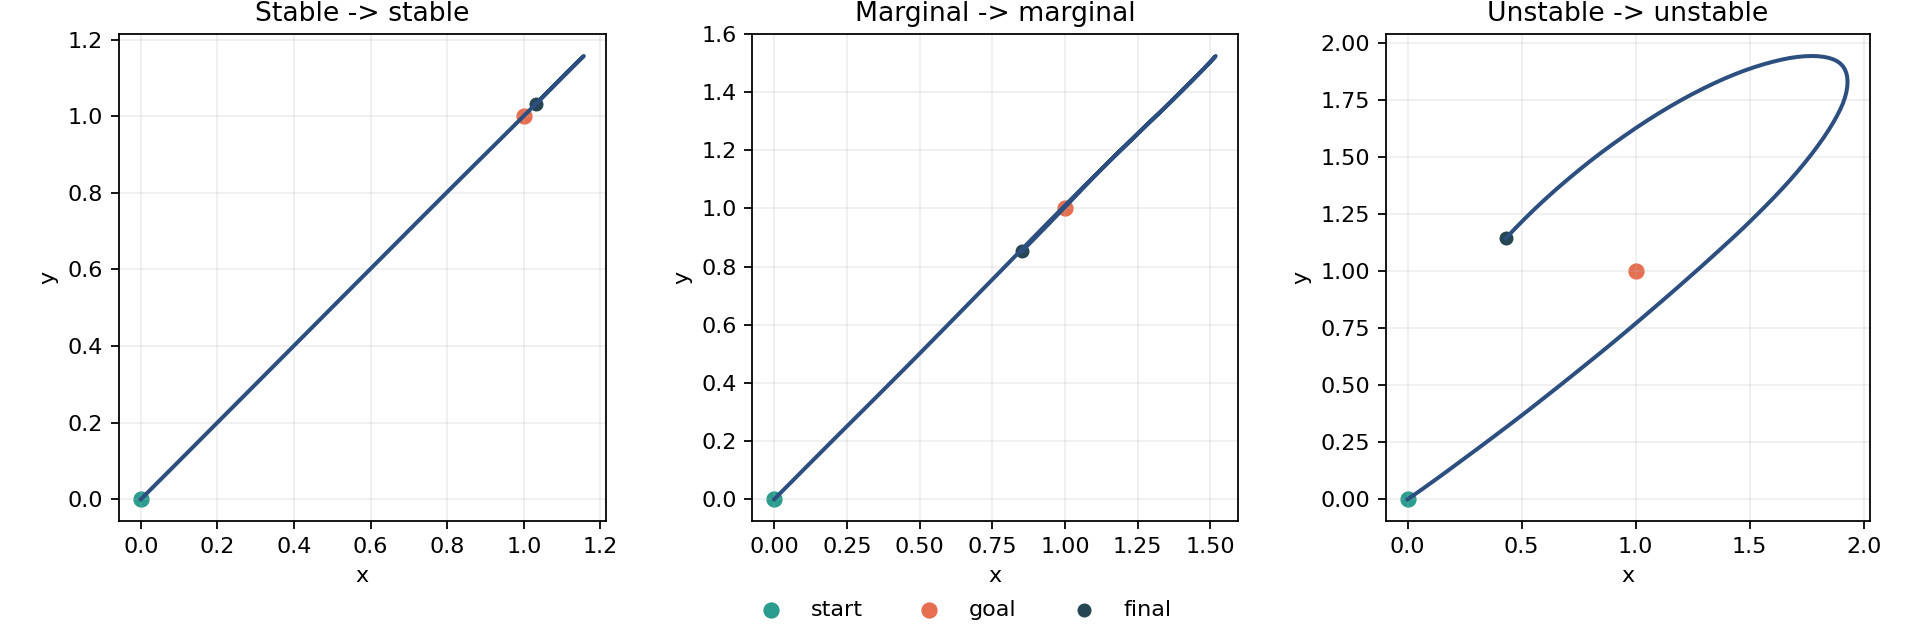
\includegraphics[width=\textwidth]{../../stability_oracle_demo_agent/output/trajectory_plot.png}
  \caption{Representative stable, marginal, and unstable agent trajectories with oracle verdicts.}
\end{figure}

\section{Interpretation}

This domain is intentionally maximally different from the first public demo:

\begin{itemize}
\item the LLM reasoning demo is symbolic and discrete
\item this demo is continuous and geometric
\end{itemize}

The point is not realism.
The point is that the same oracle can classify structural quality in both settings using the same kernel and policy surface.

\section{What This Demo Does Not Claim}

This demo does not claim:

\begin{itemize}
\item robotics competence
\item physics realism
\item control optimality
\item planning intelligence
\item universal motion safety
\end{itemize}

It only demonstrates that the Stability Oracle can classify trajectory stability in a continuous motion domain through the same reusable engine path.

\section{Operational Outputs}

The current demo generates:

\begin{itemize}
\item \texttt{results.csv}
\item \texttt{trajectory\_plot.png}
\item \texttt{DEMO\_V1\_FROZEN.md}
\item deterministic regression tests for dataset generation and regime band separation
\end{itemize}

\section{Conclusion}

This is the correct scale for the second public domain.

The demo is:

\begin{itemize}
\item small
\item deterministic
\item visually obvious
\item reusable through the same oracle kernel
\item explicit about what it does and does not test
\end{itemize}

Most importantly, it makes the decoupling claim more concrete:
the oracle is not limited to symbolic traces and can operate on continuous trajectory telemetry without changing its core semantics.

\end{document}
